\section{Exemplars}
In this section, the current IT-systems will be described and what other systems that can be used to plan what food to eat. We will find ideas from the existing systems and put them into the context of our program. \fxnote{CHS: Still don't know how to incorporate metaphors}

\subsection{Food Planner}
one technology that are currently being used to make a food plan is a mobile application called \textit{Food Planner}.
In this application the users can plan meals ahead of time, lookup recipes, look at what groceries that needs to be bought,
list what the user have in the fridge so the grocery list appends to the items in the fridge and more\fxnote{I cannot understand the last sentence..}. In the following we look at the application, to find ideas which will be good in the context of our program.\fxnote{CHS: thinks this sentence is poorly written..}

\begin{figure}[H]
    \centering
    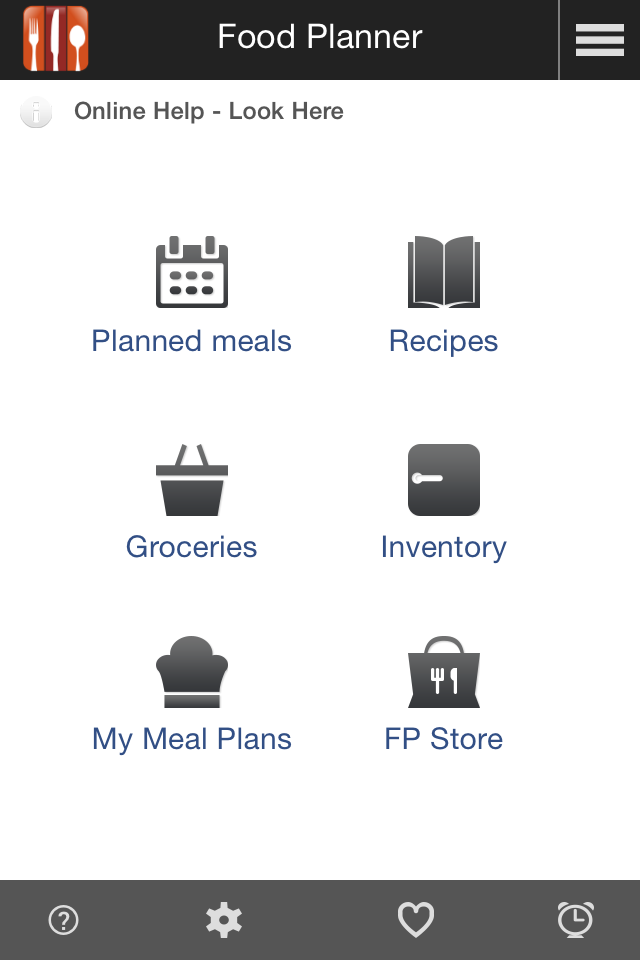
\includegraphics[width=0.5\textwidth]{Grafik/FoodPlanner/index}
    \caption{An image displaying the index of the application Food Planner}
    \label{FoodPlannerIndex}
\end{figure}

\textbf{Useful ideas:}
\begin{itemize}
  \item[Inventory:] Each product can be added separately, and the application can be used to keep track on the amount
  \item[Recipes:] Custom recipes can be created through the application, or they can be found/bought in the application store, or the internet, either by a Google search, or following a link directly to known websites, with recipes.
  \item[My meal plans:] this menu can keep track of meal planes, that has been added to the application.
  \item[Planned meals:] In this menu The upcoming days can be planed, with multiple recipes each day, either by adding them manually, or by adding a meal plan from \textit{My meal plans}. Missing groceries for a desired  number of days ahead, can then automatically be added to a \textit{Grocery menu}.
  \item[Registering:] By registering with an e-mail and a password, the application allows the user to back up the information, synchronizing with other devises and sharing is also enabled.
  \item[Grocery menu:] Here groceries that needs to be bought can be added, either automatically from \textit{My meal plan}, or added manually. If an item does not exist in the program, it can be added using a bar-code scanner.
\end{itemize}
\fxnote{Kan filføle flere billeder af FoodPlanner appen og uddube dem.}

\textbf{Idea's used in our context}

\subsection{Website}
Another alternative could be a tool found on the website madplanuge.dk\cite{madSpild_madPlanUge}. This tool is a basic foodplanner, where the foodplan can be planned one week ahead, but the users storage is taken into consideration.

When the user enters the website the user can either choose between 20 random recipes or search for something the user would like to eat.
Then the user can choose up to 3 recipes for each of the days so the user can plan breakfast, lunch and dinner for each specific day.
After the food plan has been selected, the user can then get a shopping list of all the needed items.
If the user creates a user on the site, the user will be able to save, and favorite different recipes.
If the user finds a recipe with some ingredients who the user likes, would the user be able to get more recipes based upon those ingredients.

\begin{figure}[H]
    \centering
    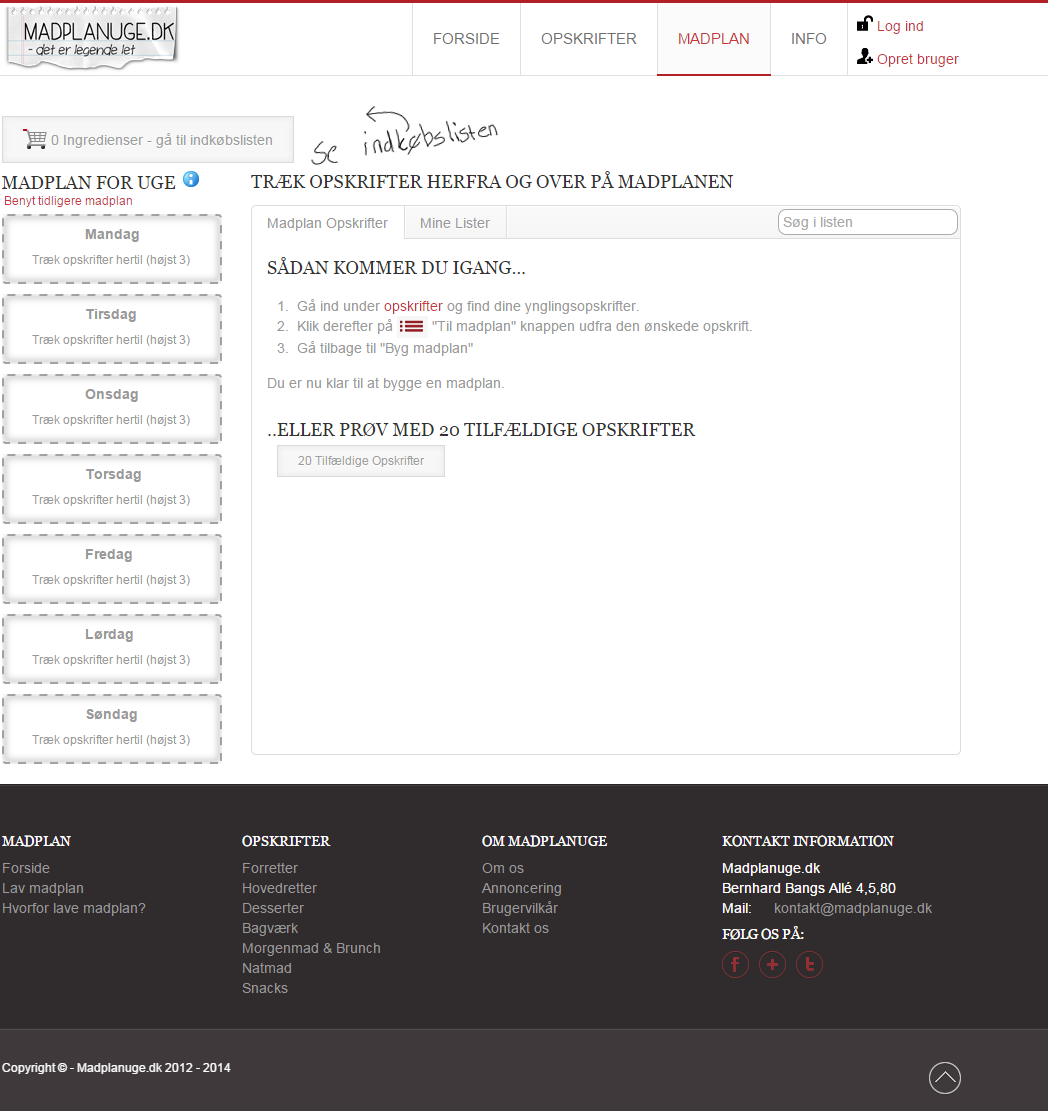
\includegraphics[width=0.5\textwidth]{Grafik/madplanuge}
    \caption{An image displaying the the website Madplan Uge}
    \label{MadPlanUge}
\end{figure}
